\documentclass{ethz_report}
\usepackage{listings}
\usepackage{color}
\usepackage{subcaption}

\definecolor{codegreen}{rgb}{0,0.6,0}
\definecolor{codegray}{rgb}{0.5,0.5,0.5}
\definecolor{codepurple}{rgb}{0.58,0,0.82}
\definecolor{backcolour}{rgb}{1,1,1}

\lstdefinestyle{mystyle}{
    backgroundcolor=\color{backcolour},
    commentstyle=\color{codegreen},
    keywordstyle=\color{magenta},
    numberstyle=\tiny\color{codegray},
    stringstyle=\color{codepurple},
    basicstyle=\ttfamily,
    breakatwhitespace=false,
    breaklines=true,
    captionpos=b,
    keepspaces=true,
    numbers=left,
    numbersep=5pt,
    showspaces=false,
    showstringspaces=false,
    showtabs=false,
    tabsize=4,
    frame=lines
}
\lstset{style=mystyle}

\title{Assignment 3 - Online Convex Programming}
\subject{Data Mining: Learning from Large Datasets}
\author{Alberto Montes}
\email{malberto@student.ethz.ch}
\date{\today}

\begin{document}
\maketitle

\section*{Problem 1: Online SVM}

For this problem is required to implement the algorithm of an Online SVM. The implementation has been done as a class encapsulating the SVM weights inside and with two methods to train from data and predict. In Listing~\ref{lst:online_svm} there is the Online SVM implementation in Python.

\lstinputlisting[language=Python, caption=Online SVM, firstline=1, lastline=28, label=lst:online_svm]{../code/online_svm.py}

To find a suitable value for $\lambda$ it has been implemented which given a model, performs a cross validation for different $\lambda$ values. For the $\lambda$ values it has been chosen to use a logarithmic scale which goes from $10^{-4}$ to $10^2$ with 30 steps. The cross validation it has been performed with 10 folds. On Listing~\ref{lst:cv_function} there is the code function to compute this results.

\lstinputlisting[language=Python, caption=$\lambda$ computation with CV, firstline=77, lastline=121, label=lst:cv_function]{../code/online_svm.py}

Then, in order to compute the classification error of the test set depending to the number of samples used to train, a function has been written which trains the same model with different number of samples and plot the results. On Listing~\ref{lst:train_function} there is the correspondent code.

\lstinputlisting[language=Python, caption=Computation of the classification error vs. samples used for training, firstline=123, lastline=153, label=lst:train_function]{../code/online_svm.py}

To run all this code it is only necessary to give the \texttt{OnlineSVM} class previously created to the previous functions. To find the suitable value of lambda I have obtained the following results. On Figure~\ref{fig:cv_lambda} there is plot for each value of $\lambda$ the classification accuracy for a cross validation of 10 folds as well as the classification accuracy error.

\begin{figure}[H]
\centering
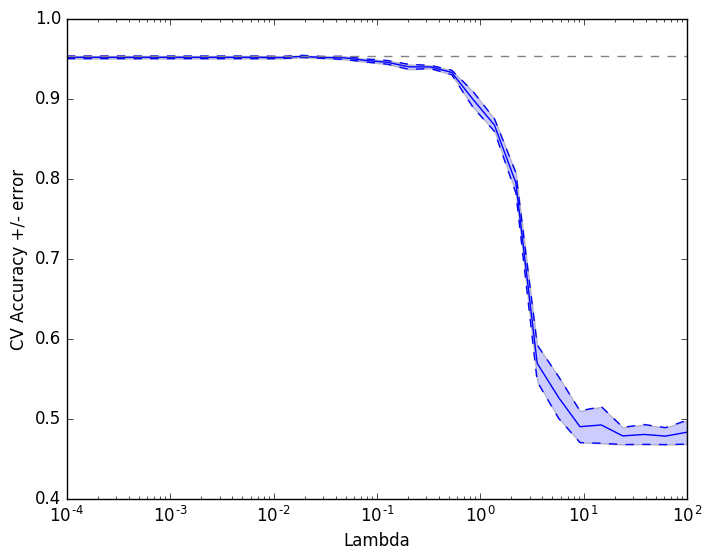
\includegraphics[width=.85\linewidth]{./img/cross_val_svm.png}
\caption{Classification Accuracy for different values of $\lambda$}
\label{fig:cv_lambda}
\end{figure}

It can be seen haw at values of $\lambda < 10^{-1}$ the classification accuracy stays constant and maximum while for values of $\lambda > 10$ the classification is around 50\%. The best result is found with $\lambda = 0.01$ and gives an accuracy of 95.79\%.

On the experiment representing the classification error versus the number of samples used to train, on Figure~\ref{fig:ce_vs_samples_svm} there is the results presented. The experiment has been made with the value of $\lambda = 0.01$ as it performs the best classification accuracy.

\begin{figure}[H]
\centering
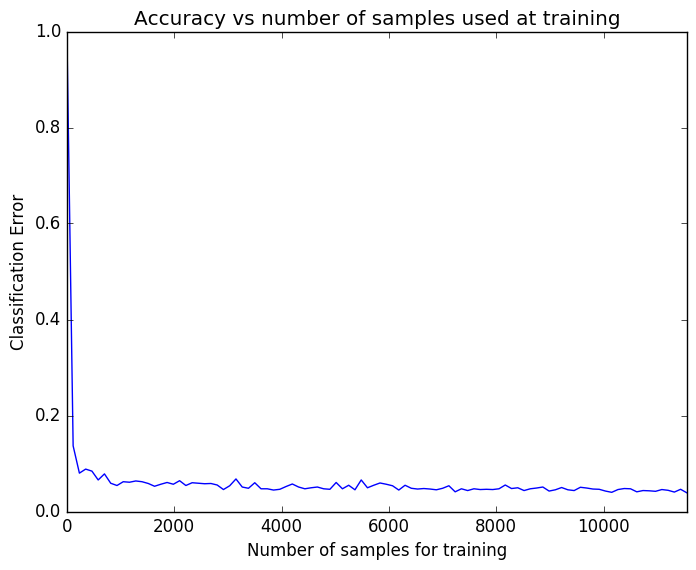
\includegraphics[width=.85\linewidth]{./img/acc_vs_samples_svm.png}
\caption{Classification Error vs samples used to train }
\label{fig:ce_vs_samples_svm}
\end{figure}

It can be seen how with a few samples for training, the Online SVM model converge into the final classification error, so the total number of samples available is larger than required to train the model.

\section*{Problem 2: Online Logistic Regression}

For the Problem 2, it was required to perform the same computations than in Problem 1 but implementing the algorithm for an Online Logistic Regressor. For this case, as the loss function and restriction is different. For the logistic regression the loss is logarithmic and the restriction depends on norm $L_1$ so the weights update will be as follows:

\begin{equation}
    w_{t+1} := w_t + \eta_t \frac{y_t \mathbf{x}_t}{1 + \exp(y_t \mathbf{w}^T_t \mathbf{x}_t)}
\end{equation}

The resulting implementation of the Online Logistic Regression is in the Listing~\ref{lst:online_log_reg}.

\lstinputlisting[language=Python, caption=Online Logistic Regression, firstline=30, lastline=49, label=lst:online_log_reg]{../code/online_svm.py}

To find the best value of $\lambda$ it has been performed the same computations than in Problem 1 but using the previous presented model. The accuracy along different values of $\lambda$ can be found on Figure~\ref{fig:cv_lambda_reg}.

\begin{figure}[H]
\centering
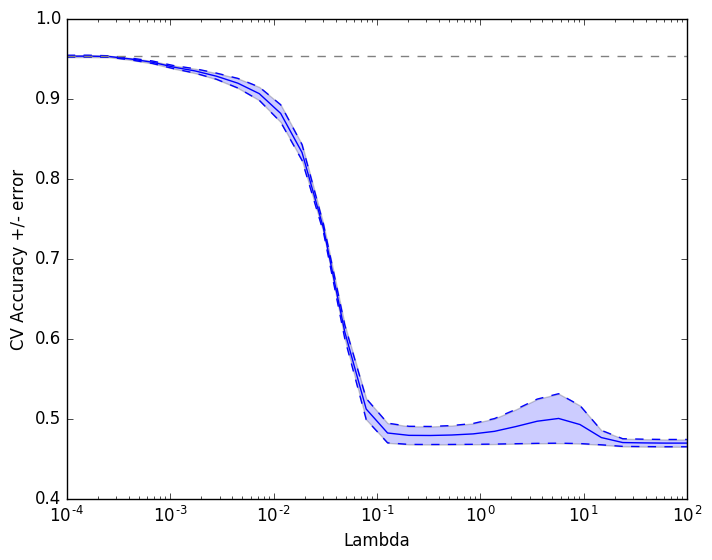
\includegraphics[width=.85\linewidth]{./img/cross_val_logistic.png}
\caption{Classification Accuracy for different values of $\lambda$}
\label{fig:cv_lambda_reg}
\end{figure}

As can be seen, the best results are achieved with lower value of $\lambda$ than in the Online SVM. For $\lambda < 10^{-4}$ it is achieved the maximum accuracy, while for $\lambda > 10{-1}$ the accuracy seem to be random. The best accuracy, achieved with $\lambda = 10^{-4}$ has been 96.21\%.

Finally, the classification error of the best model found with $\lambda=10^{-4}$ has been computed for different number of samples used to train. In Figure~\ref{fig:ce_vs_samples_logistic} there is the results.

As happened with the Online SVM, the number of samples needed to converge on the minimum classification error are very few (only approximately 500).

\begin{figure}[H]
\centering
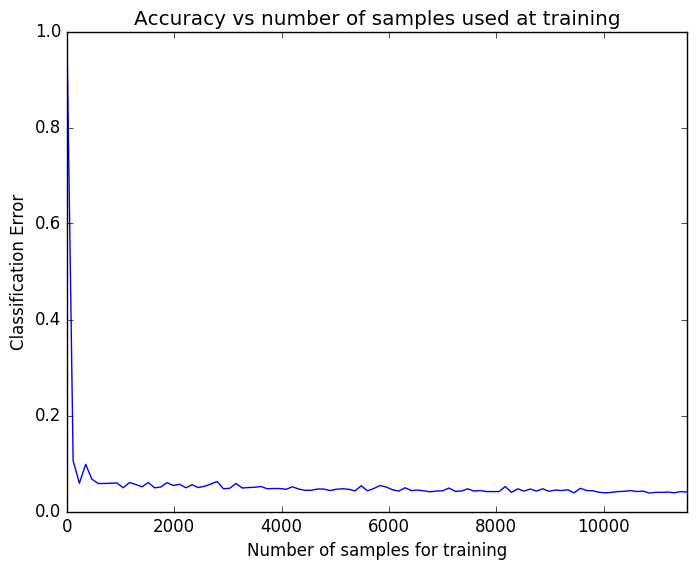
\includegraphics[width=.85\linewidth]{./img/acc_vs_samples_logistic.png}
\caption{Classification Error vs samples used to train}
\label{fig:ce_vs_samples_logistic}
\end{figure}

\end{document}
